\documentclass{ximera}

\begin{document}
\begin{problem}
  Four numbers $A$, $B$, $C$, and $D$ are shown below on a number line.
  \begin{image}
  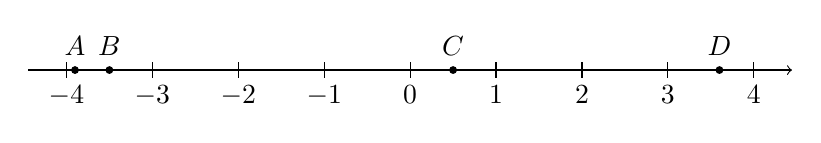
\begin{tikzpicture}[x=0.09\textwidth]
    \draw[-{>[scale=1.75]}] (-0.4\textwidth,0) -- (0.4\textwidth,0);
    \foreach \x in {-4,...,4} {%
      \draw (\x,-.1) -- (\x,.1);
      \node[anchor=north,yshift=-2pt] at (\x,0) {$\x$};
    }
    \draw (-3.9,0) node [circle,fill,inner sep=1pt,label=above:$A$](e){};
    \draw (-3.5,0) node [circle,fill,inner sep=1pt,label=above:$B$](e){};
    \draw (0.5,0) node [circle,fill,inner sep=1pt,label=above:$C$](e){};
    \draw (3.6,0) node [circle,fill,inner sep=1pt,label=above:$D$](e){};
  \end{tikzpicture}
  \end{image}
  Which is closest to the average of $A$, $B$, $C$, $D$?
  \begin{multipleChoice}
    \choice{$A$}
    \choice{$B$}
    \choice[correct]{$C$}
    \choice{$D$}
  \end{multipleChoice}
\end{problem}
\end{document}
